\documentclass{article}
\title{Atreus Keyboard Assembly}
\date{ }
\usepackage{graphicx}
\begin{document}
\setlength{\parindent}{0cm}
\maketitle
\section{Prerequisites}

In order to assemble your keyboard, you'll need your kit plus a few
other tools. The kit should contain these parts and a few spares:

\begin{itemize}
\item Case (top plate, switch plate, spacer, bottom plate)
\item Sandpaper
\item Finishing wax
\item Diodes (42)
\item Cherry MX switches (37 blue/clear, 5 red)
\item A-Star Micro controller
\item Machine screws and nuts (8 each, 16mm M3 size)
\item Key caps (40 normal, 2 long)
\item USB micro cable
\item Rubber feet
\end{itemize}

You'll also need to have these on hand:

\begin{itemize}
\item Soldering iron and solder
\item Wire cutters
\item Brush for applying finishing wax (a toothbrush will do)
\item Optional: ``helping hands'' stand
\end{itemize}

\vspace{1em}

The latest version of this document can always be found
online.\footnote{http://atreus.technomancy.us/assembly.pdf} If you're
reading a black-and-white printed copy, you may find some of the
photos clearer in color onscreen. This copy describes
the circuit-board-based kit. If you have an earlier hand-wired kit,
see the older assembly
guide.\footnote{http://atreus.technomancy.us/assembly-hand-wired.pdf}

\section{Sanding Case}

The wood finishing process involves sanding down the wood to remove
scorch marks and produce a smooth surface, applying an oil/wax mixture
to further smooth it and protect it from fluids, and allowing it to
dry. The whole process takes about 45 minutes of work, but since each
side has to dry individually plan on allowing for a couple 30-minute
breaks to let it dry. You'll need a place to lay the pieces aside to
dry; a paper towel would help keep the oil from getting all over your
table or desk.

\vspace{1em}

Start by sanding down both sides of each piece. You may want to hold
two pieces together while sanding for strength or placing it on a flat
surface you don't mind scruffing up; too much pressure on a single
plate could damage it.

\vspace{1em}
\noindent\makebox[\textwidth]{%
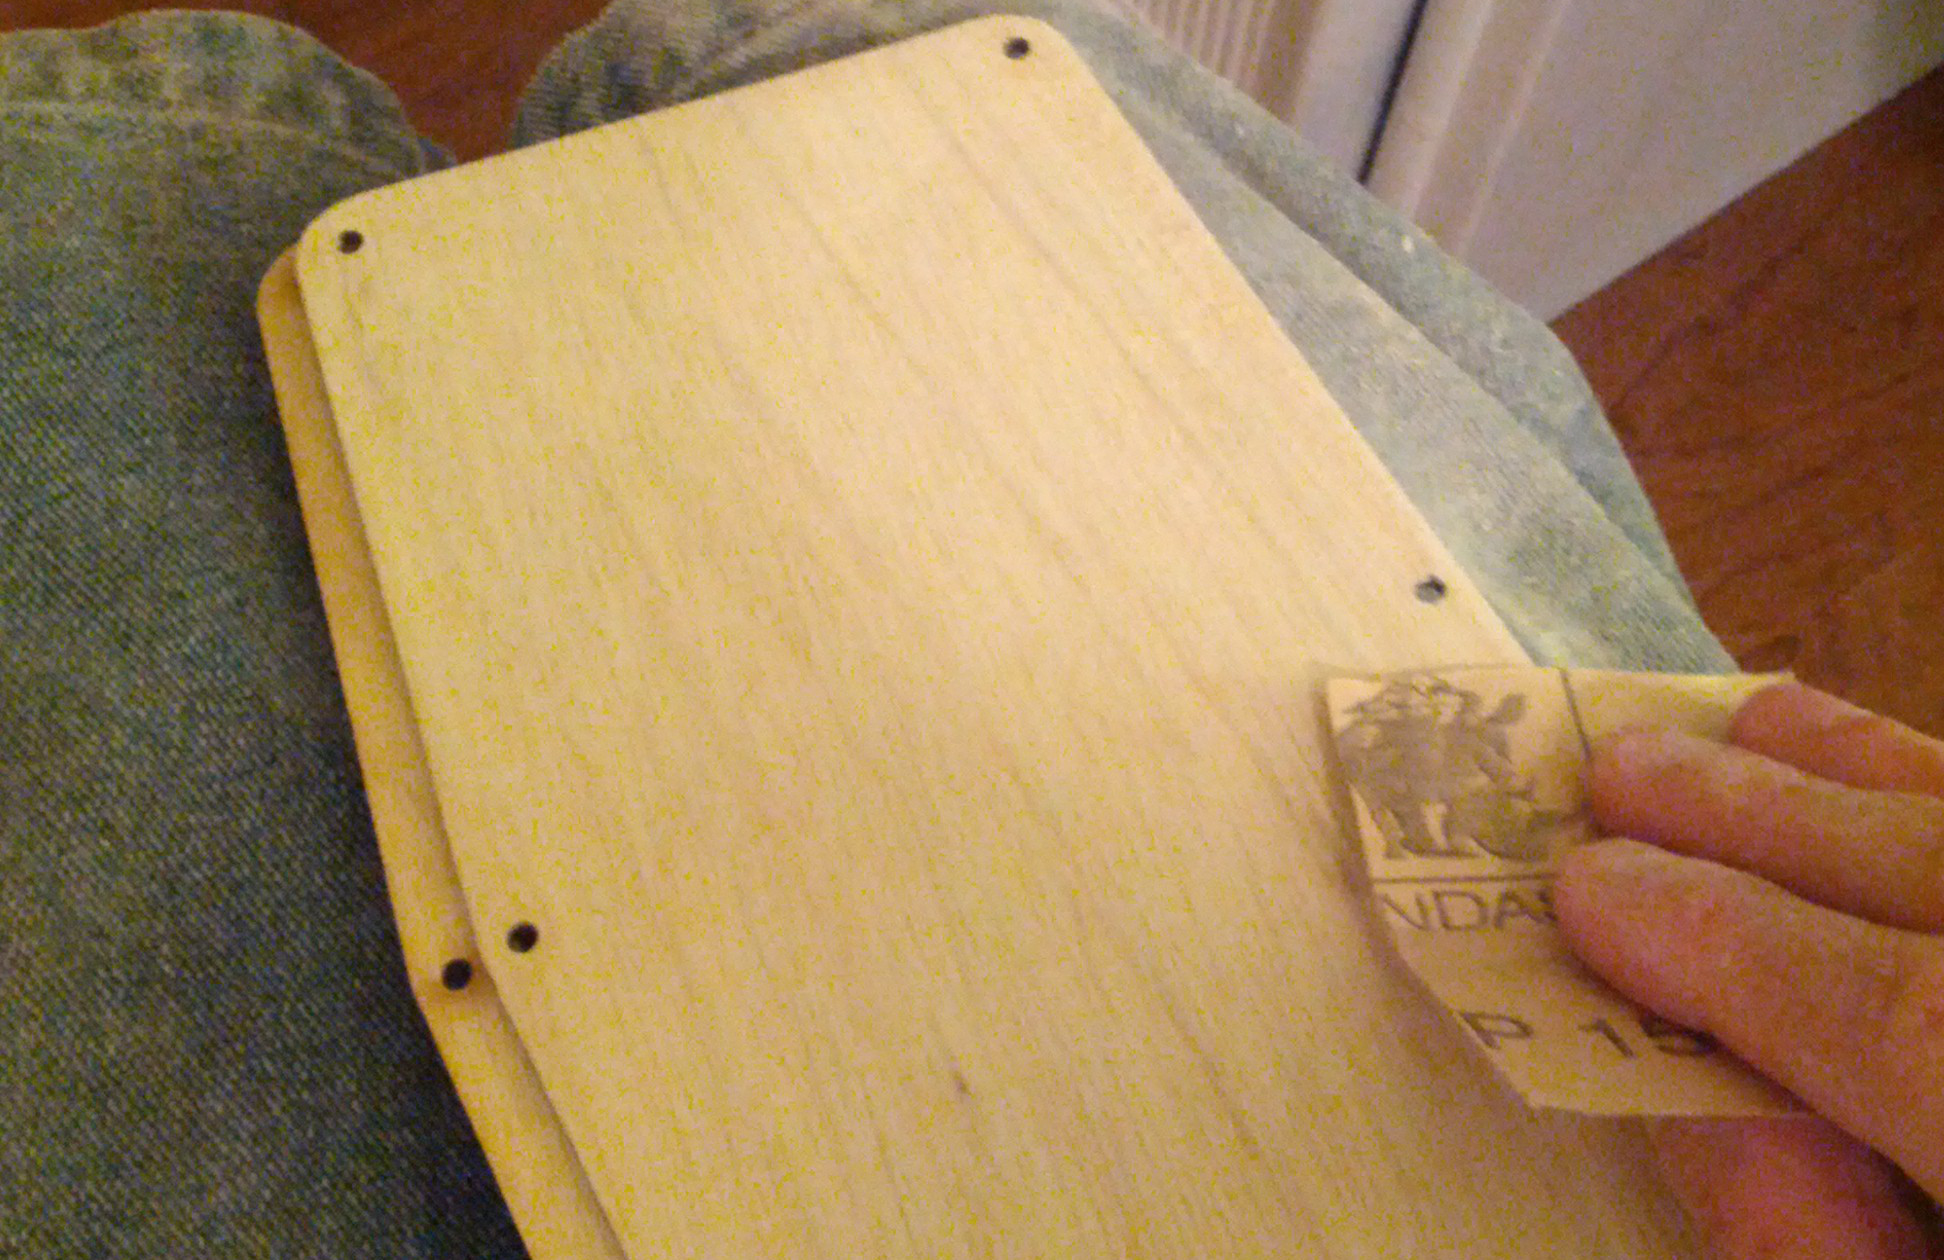
\includegraphics[width=\linewidth]{sanding.jpg}}
\vspace{1em}

Keep in mind that the top side of the top plate and the bottom side of
the bottom plate are the only surfaces that are exposed to the touch
once the keyboard is fully assembled, so these will need the most
attention when sanding. You can sand the other surfaces as well just
to get the scorch marks off, but you don't need to worry about how
smooth the inner surfaces feel to the touch.

\section{Oiling Case}

Be sure to get all the wood dust off the pieces before you go on. Open
up the wax/oil mixture. Dip your brush in and start spreading it over
one side of each case piece. The color of the wood will darken as it
absorbs the oil. Try to ensure it's spread evenly. Be more generous
with the oil on the outer exposed surfaces.

\vspace{1em}
\noindent\makebox[\textwidth]{%
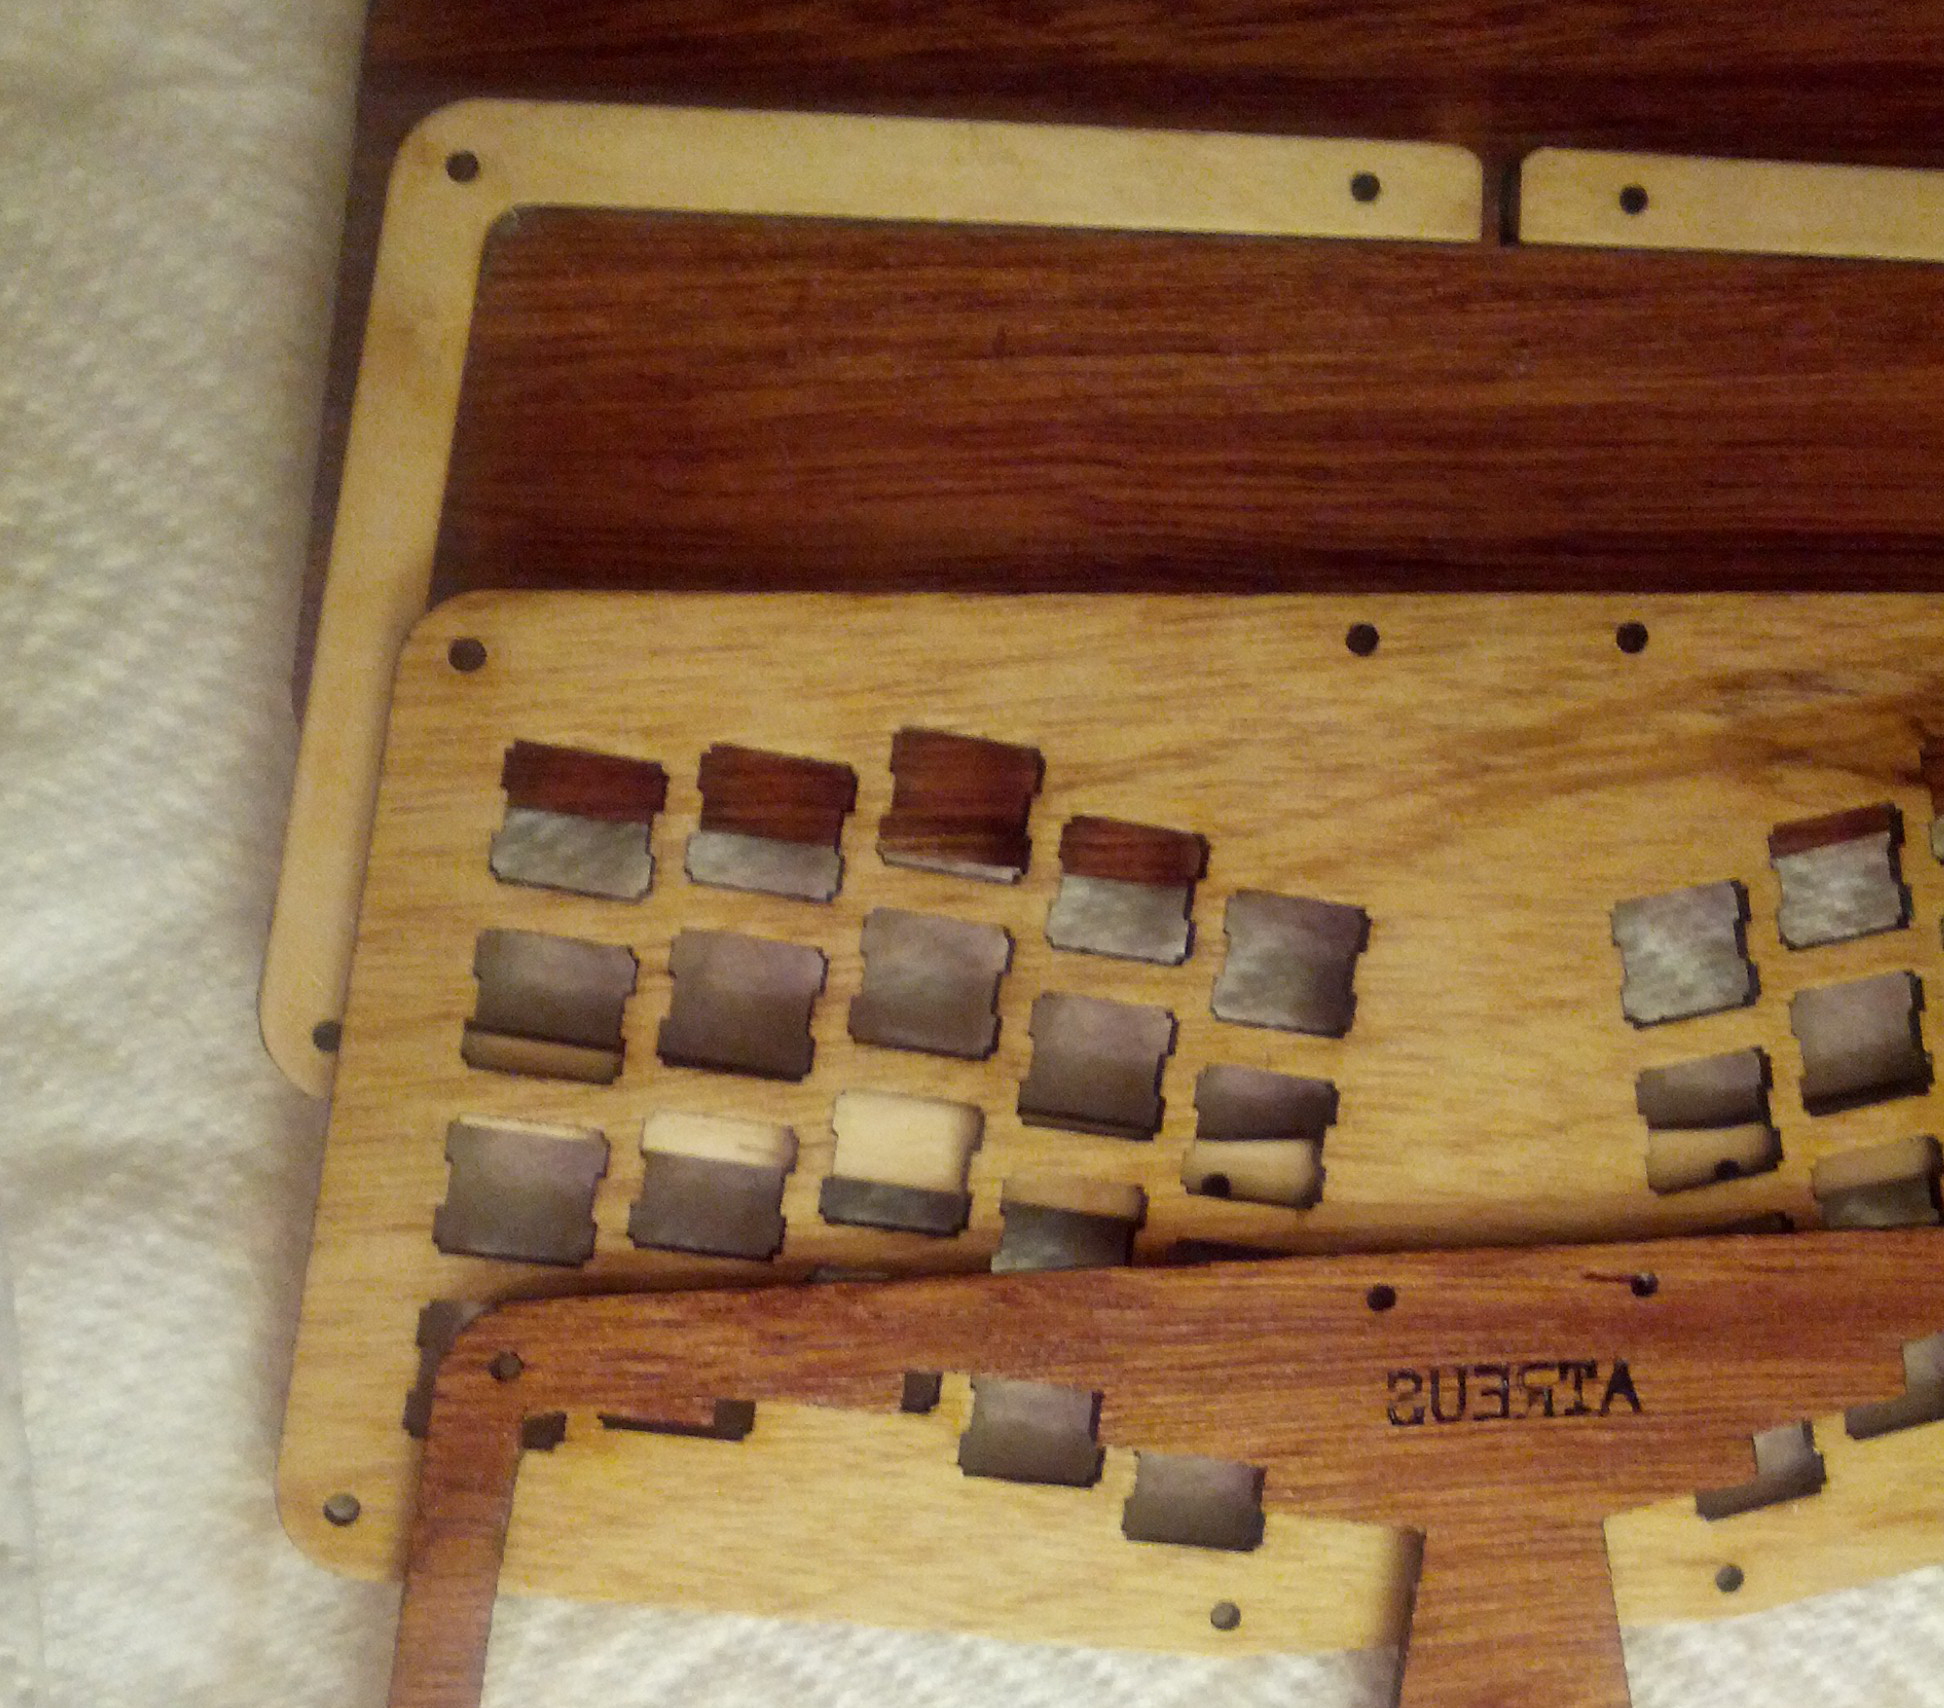
\includegraphics[width=\linewidth]{oiled.jpg}}
\vspace{1em}

As your brush goes over the edges of the laser-cut wood, it will get
dirty from charred wood particles. After you've finished oiling one
side of each piece, it's best to wash out the brush. Be sure it's
fully dry before going on.

\section{Drying Case}

Once one side of each piece is finished, you'll need to lay them out
for a half hour or so to let them dry. Once one side is dry, repeat
the process on the other side. After you've finished all the soldering
you can come back and add another few coats to the outermost surfaces
for a smoother texture. Once it's dried for a while, wipe the excess
off. While you're waiting, you can start soldering the diodes and
controller onto the circuit board, but don't solder any switches in
before the switch plate is ready or you'll just need to remove them
later.

\section{Diodes}

If you've never soldered before, there are plenty of good
introductions online.\footnote{This one from Adafruit is great:
  https://learn.adafruit.com/adafruit-guide-excellent-soldering/tools}
Coat the tip of the iron thinly with some solder before you start. The
key is to use the iron to heat the joint for a second or two, then
bring in a dab of the solder and let it melt and stick to the
component and the circuit board pad.

\vspace{1em}

Take five diodes at a time and bend them into a U shape. Place them
into the diode holes next to each switch slot on the reverse side of
the board. Each diode has a black band on it; the band should be
pointing to the bottom of the circuit board, toward the arrow on the
board. Bend the legs of the diodes outwards to hold them in place,
then flip the board over and solder them in place.

\vspace{1em}
\noindent\makebox[\textwidth]{%
  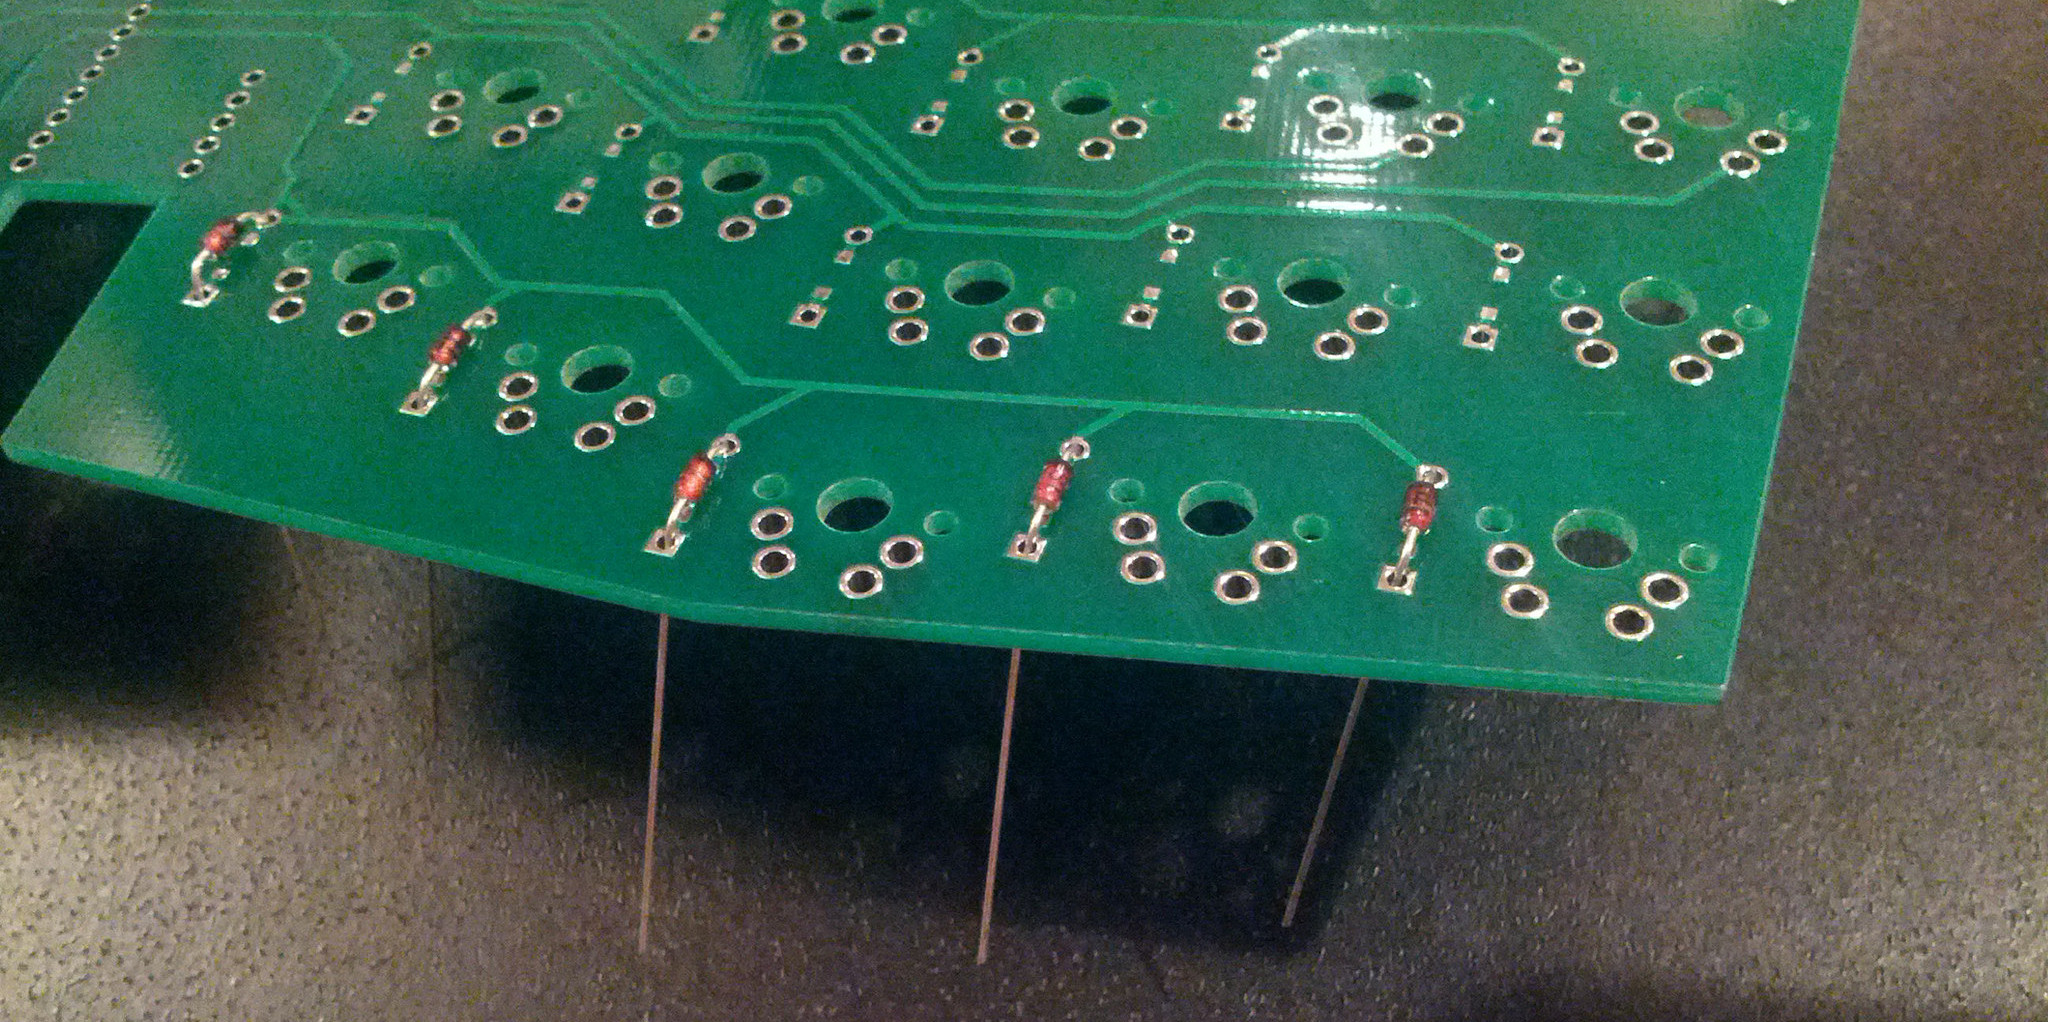
\includegraphics[width=\linewidth]{diodes.jpg}}
\vspace{1em}

Once they're soldered, trim the diode legs with wire
cutters. (This step should be done with protective eye covering.) Keep
the diode legs; they will be needed in the next step.

\section{Controller}

Once the diodes are in place, you can begin attaching the
controller. This is the trickiest part of the assembly process, so
once you knock this out it's all down hill. First pre-fill all the
holes we're going to use on the controller with solder. (This is all
the left side ones, plus all the right side ones except 3V3, 5V, and
VIN.) If you have a ``helping hands'' stand, this is where it comes in
useful.

\vspace{1em}

Take six trimmed diode legs and stick them into the top six pins on
the right-hand side of the controller by melting the pre-filled
solder. Solder one into the pin labeled ``GND'' as well. Put one in
the top and bottom pins on the other side, labeled ``0'' and
``9''. We'll leave out the rest on the left for now to make
it easier to insert the controller into the circuit board, but we'll
make another pass to get those in next.

\vspace{1em}
\noindent\makebox[\textwidth]{%
  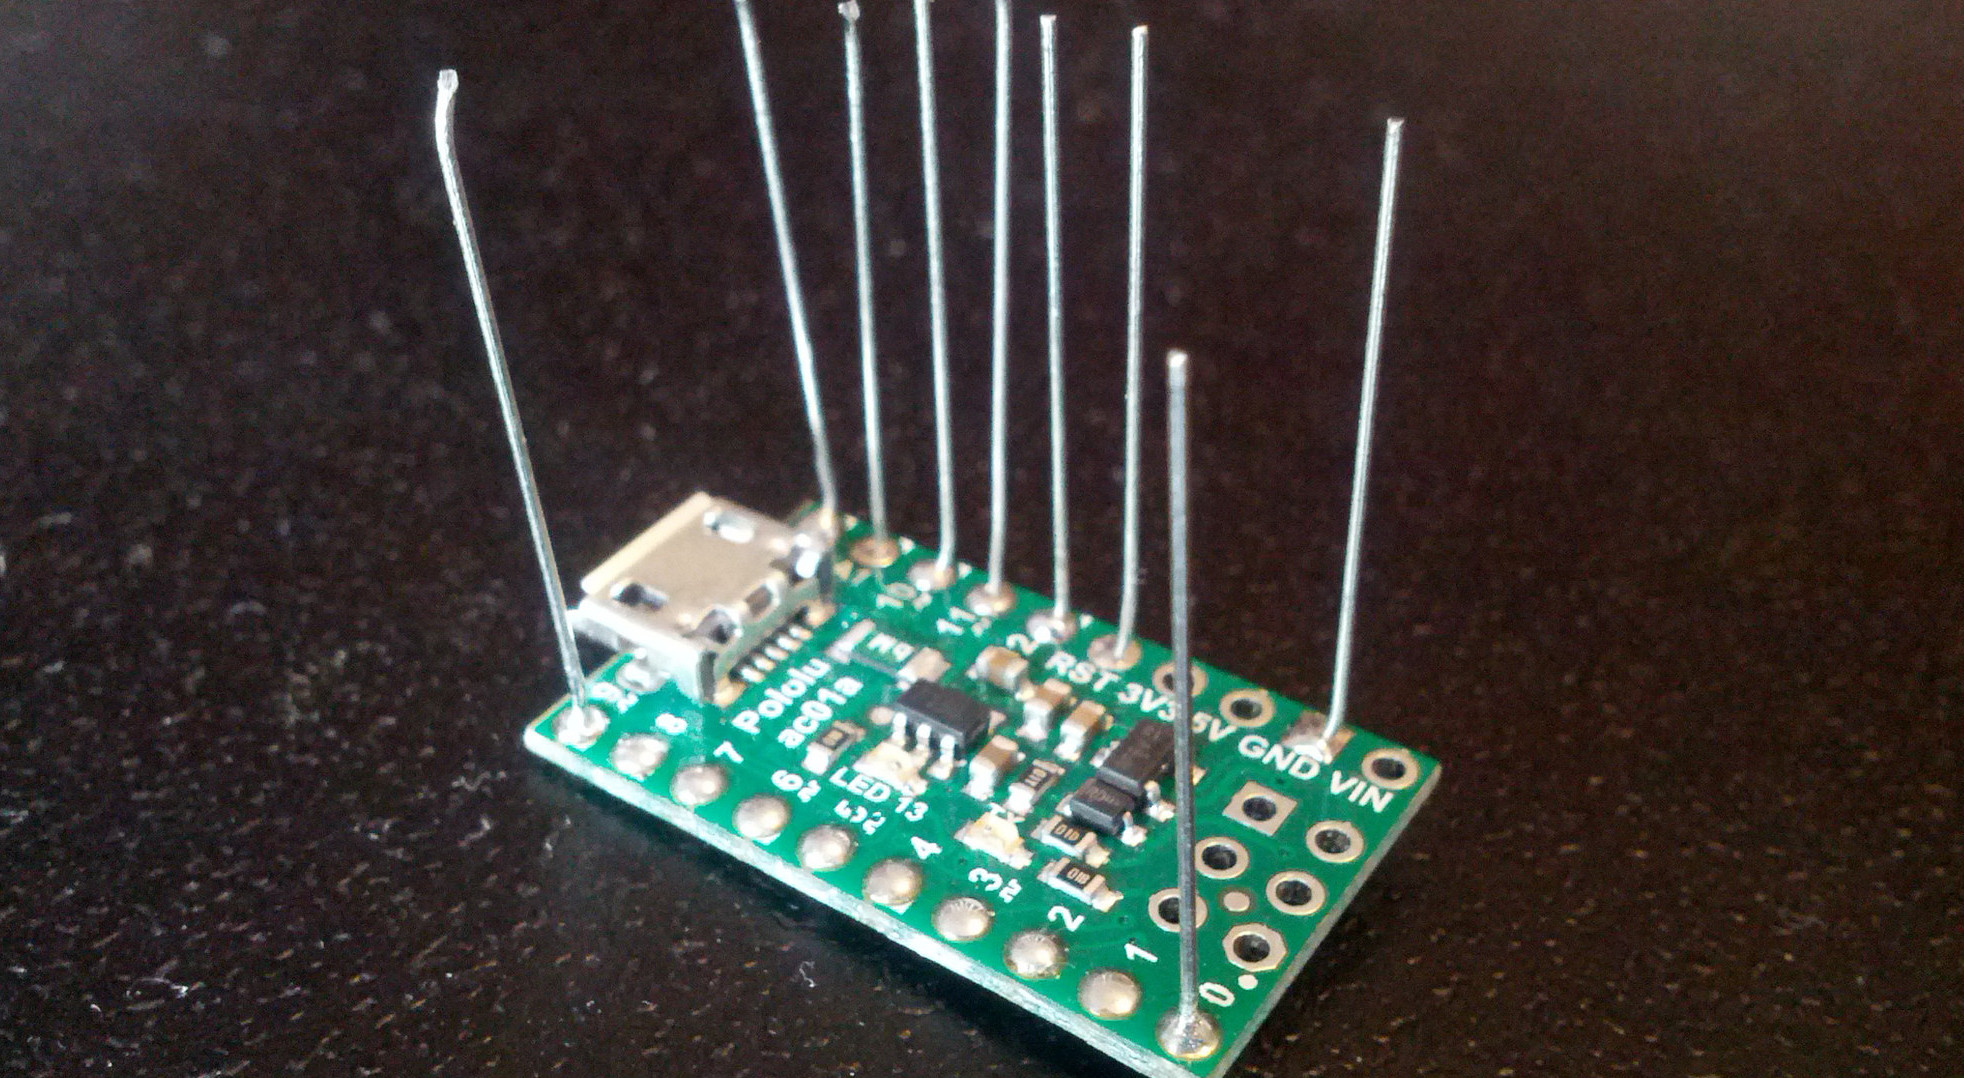
\includegraphics[width=\linewidth]{controller-legs.jpg}}
\vspace{1em}

Straighten the attached legs as much as possible and carefully insert
them through the circuit board. Once they are in, you'll want to
populate the remaining left-side pins. Hold the board vertical either
using a set of helping hands or pinned between your knees as shown
below. Insert a diode leg through the circuit board hole so it touches
the already-solder-filled hole on the controller. Melt the solder
while pushing the diode leg barely through. You can blow on the solder
joint to cool it more quickly so it firms up.

\vspace{1em}
\noindent\makebox[\textwidth]{%
  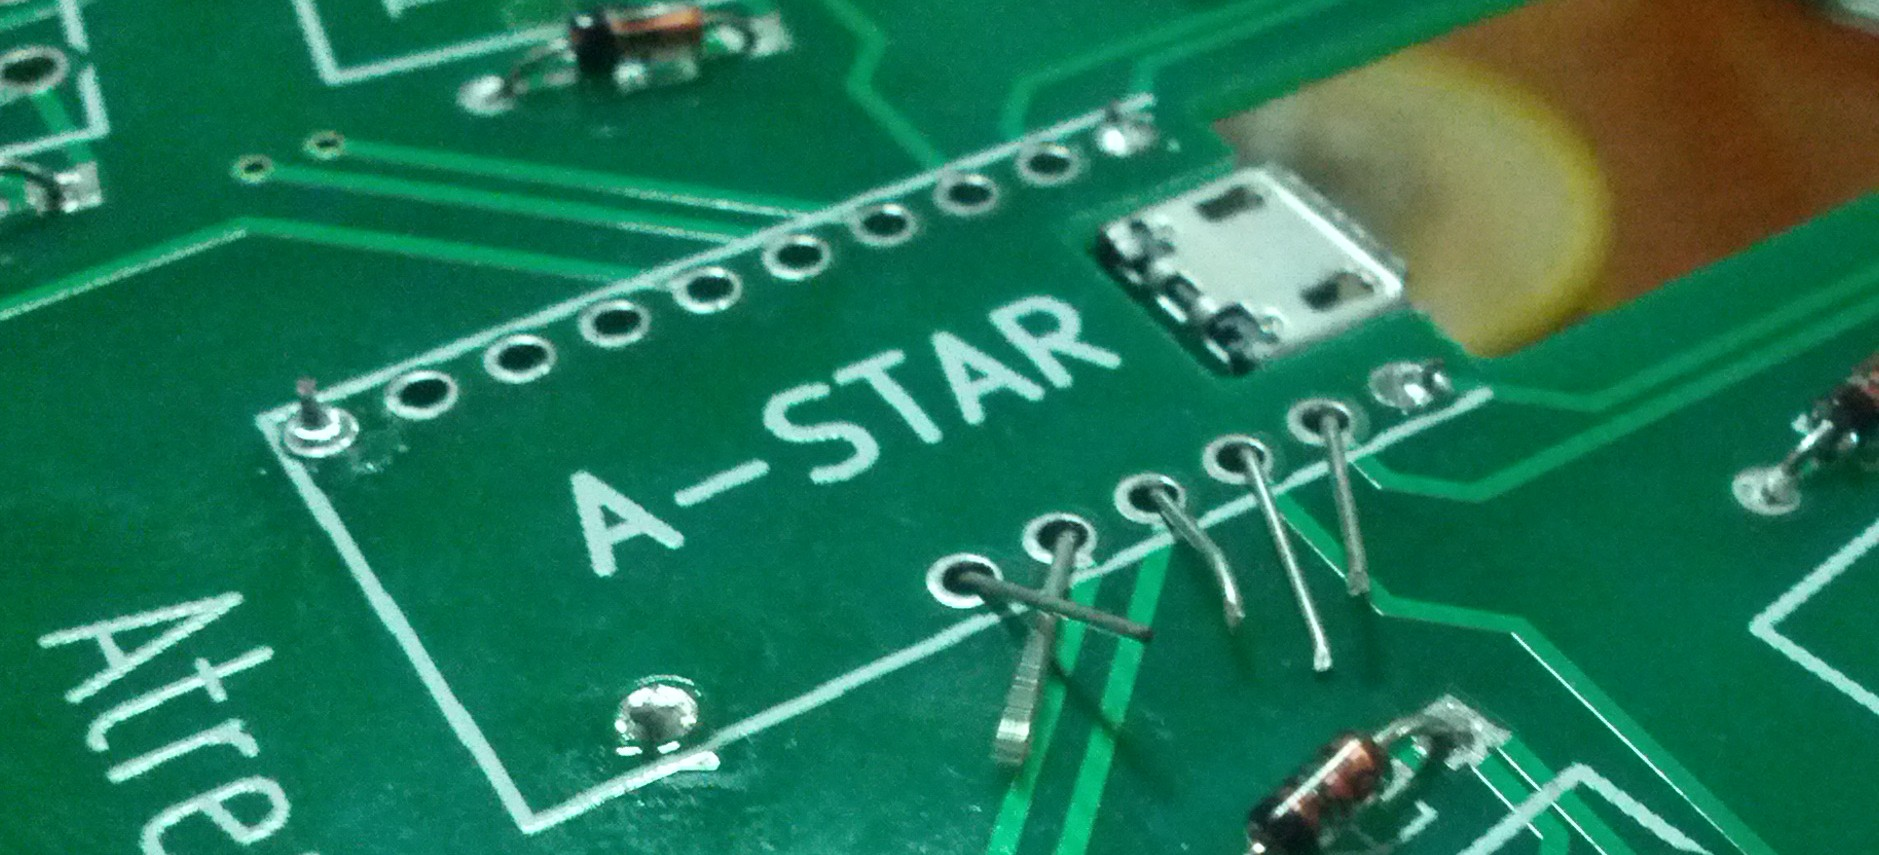
\includegraphics[width=0.5\linewidth]{insert-pin.jpg}}
\vspace{1em}

Once the pins are all in place on the controller side, it's time to
attach them to the circuit board. Bend them outwards and solder each
one, then trim all the legs.

\vspace{1em}
\noindent\makebox[\textwidth]{%
  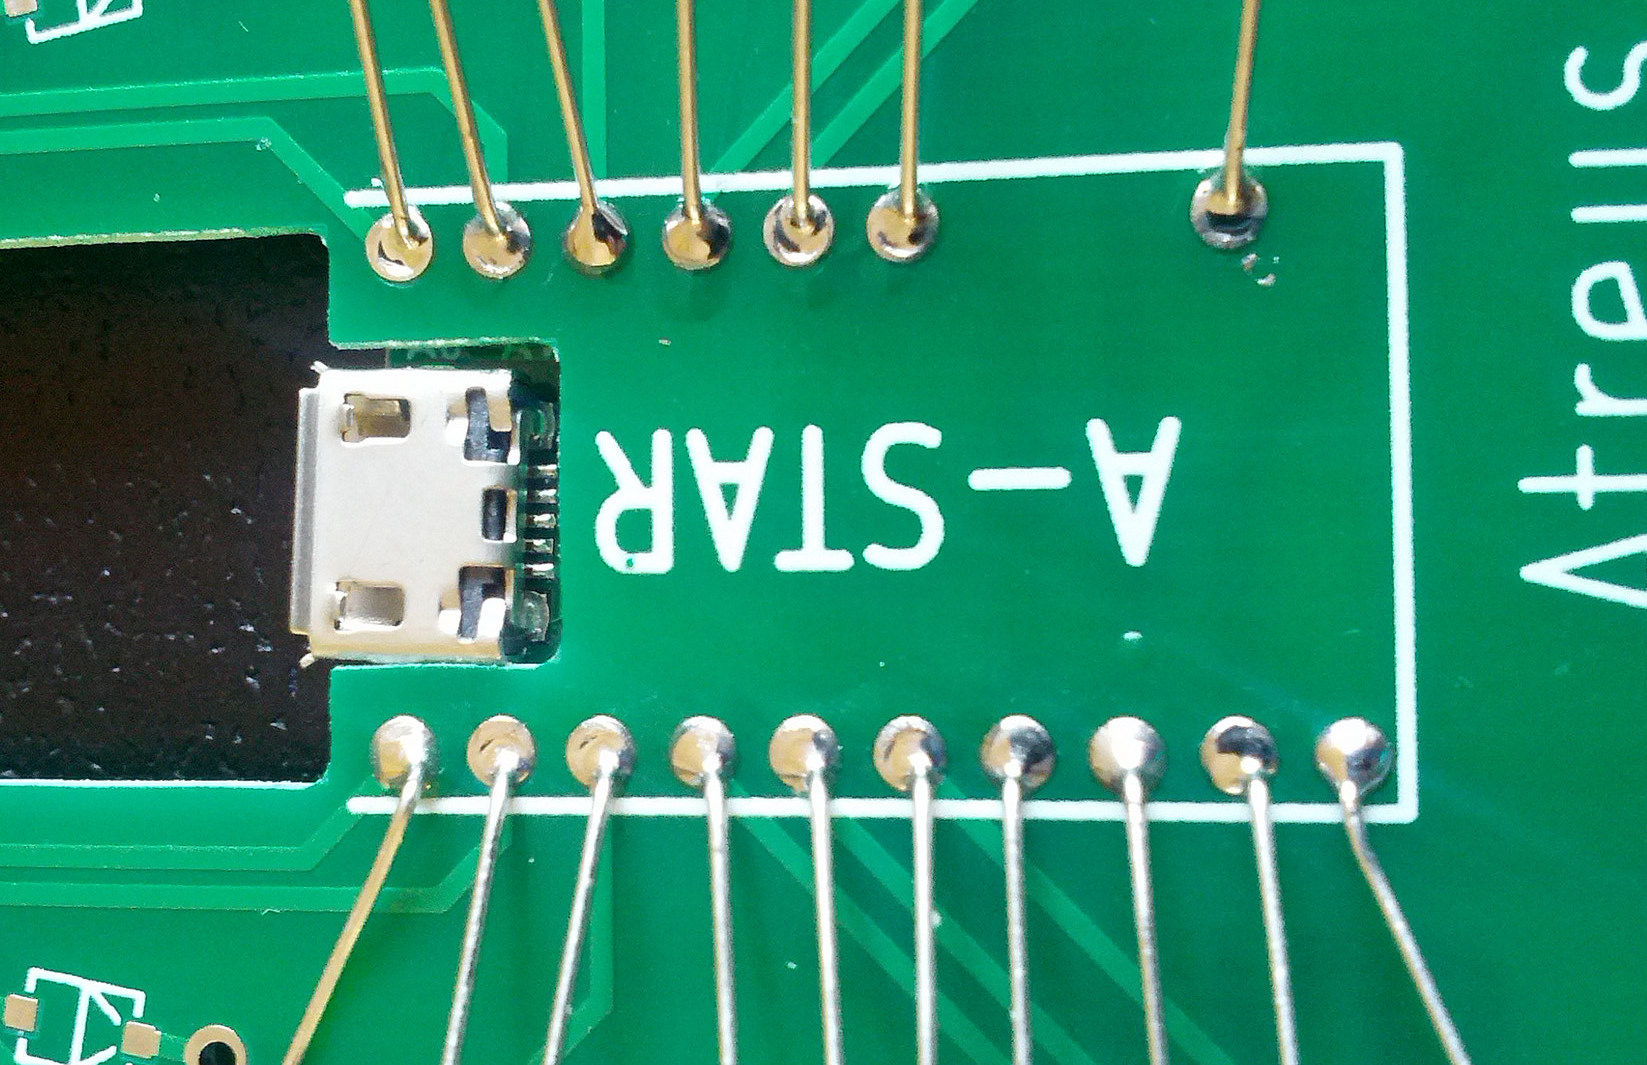
\includegraphics[width=\linewidth]{seated.jpg}}
\vspace{1em}

Before you go on, take the time to double-check the solder joints on
the controller. The solder should fill the hole completely without
spilling over to adjacent holes, and the legs should be secure. Also
check that all the diodes are facing the correct direction with the
black band on the bottom side. Once the switches are in place, the
controller will be pinned between the switch plate and the circuit
board, making it difficult to make further changes to the controller.

\section{Switches}

\noindent\makebox[\textwidth]{%
  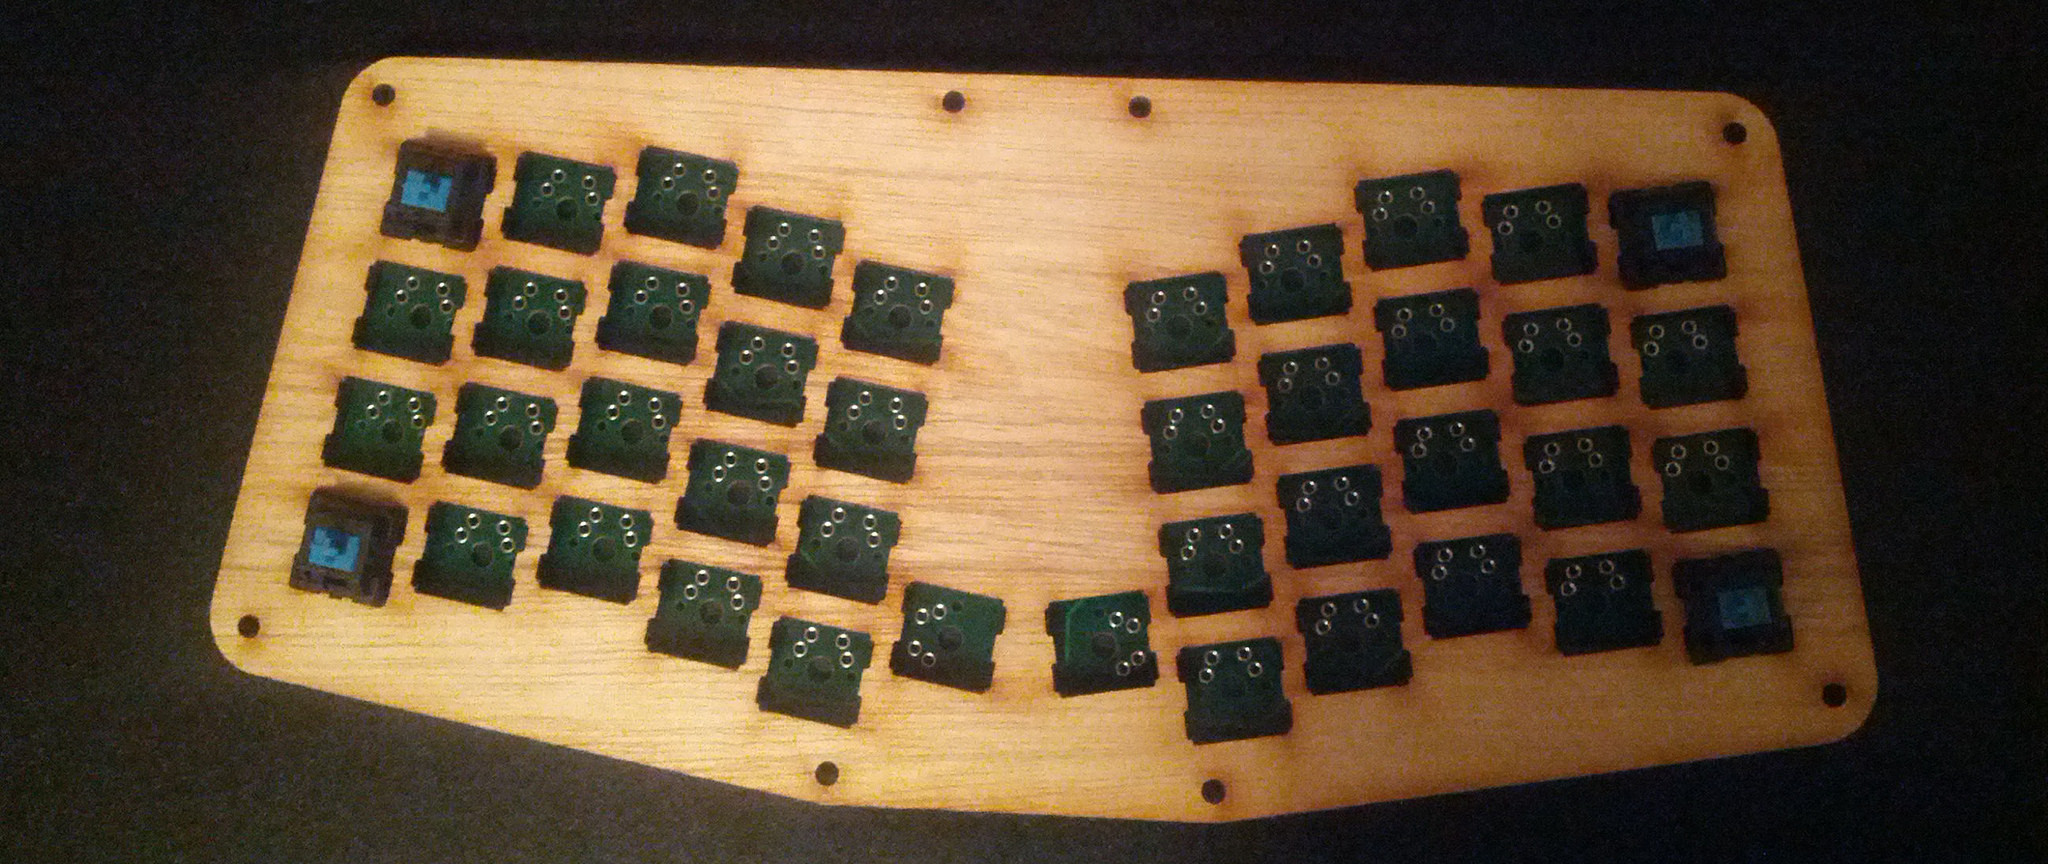
\includegraphics[width=\linewidth]{switch-corners.jpg}}

\vspace{1em}

Next take four switches and place each switch in a corner of the
switch plate. Put the switch plate face-down on the table with the
pins sticking up. Carefully fit the circuit board over the protruding
pins and posts and solder those to hold the circuit board and the
switch plate together. The labeled side of the board should be
face-up. Take care that the switch pins are straight; pushing in a
switch with a pin that's a bit bent will bend it flat and prevent it
from poking through the circuit board.

\vspace{1em}

If your kit has five linear switches (non-tactile, usually red) place
those in the modifier positions next and solder them in. These all go
on the bottom row: SW3:3, SW5:0, SW6:0, SW8:3, and SW9:3. Then proceed
with the rest of the switches. The switches should pin the switch
plate to the circuit board.

\vspace{1em}
\noindent\makebox[\textwidth]{%
  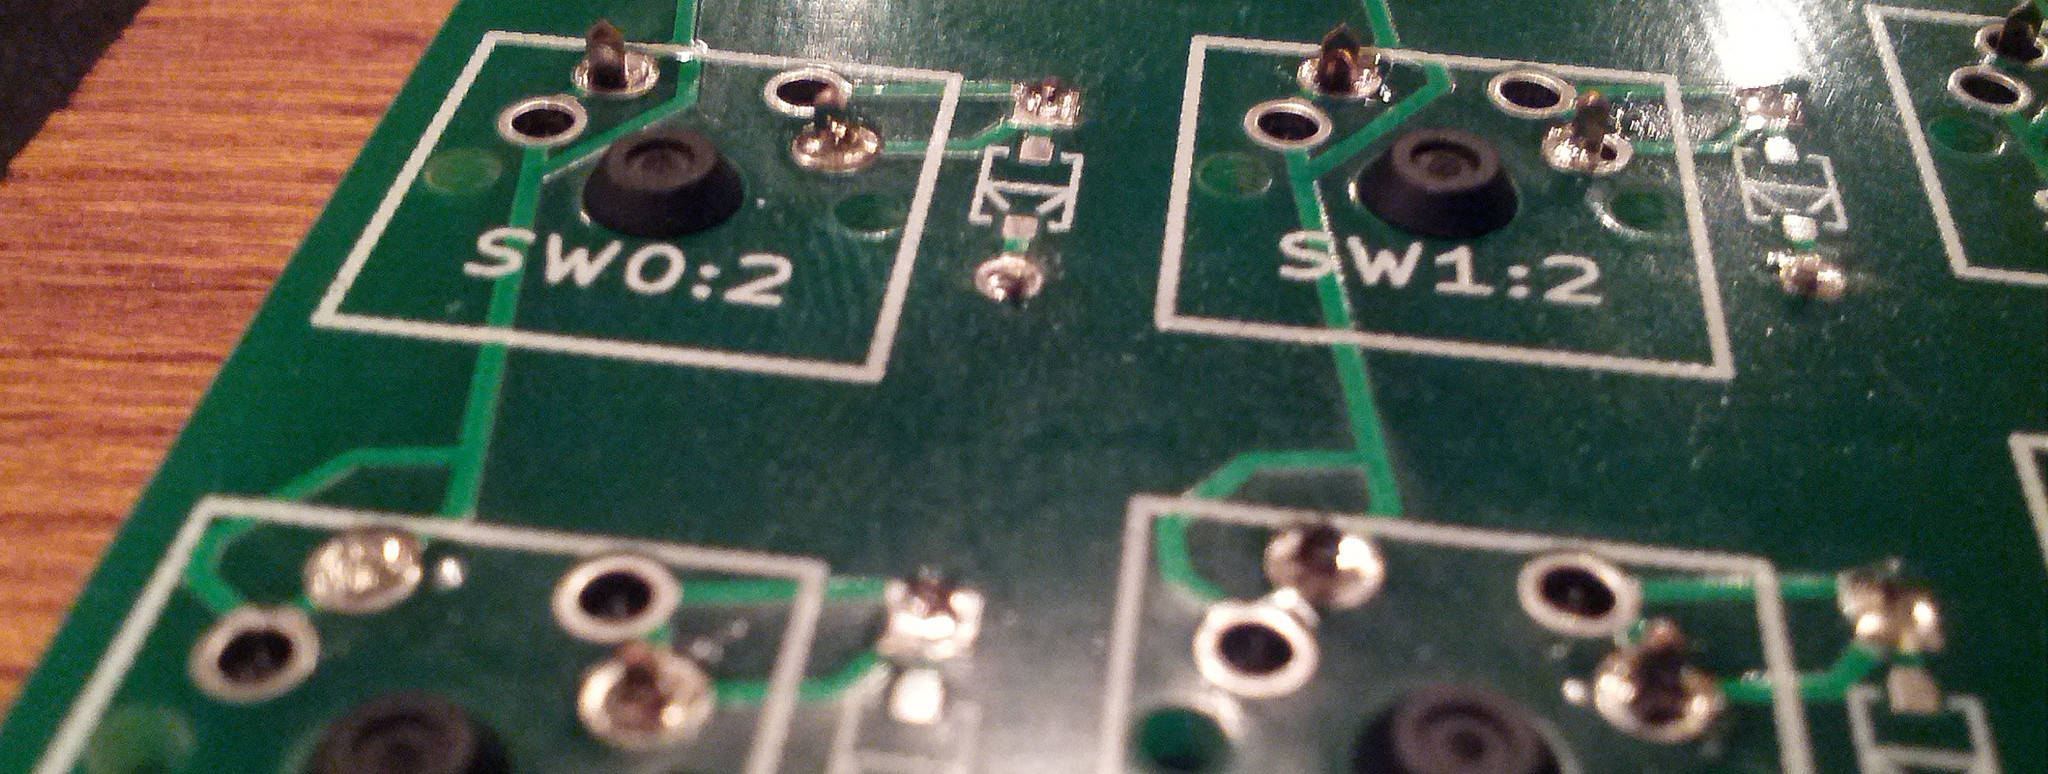
\includegraphics[width=\linewidth]{switches.jpg}}
\vspace{1em}

\section{Wrapping up}

Plug in the USB micro cable into the controller, and plug the other
side into your computer. Get a copy of the
firmware \footnote{Available at
  https://github.com/technomancy/atreus-firmware} and its
dependencies, \texttt{avrdude} and \texttt{gcc-avr}, linked in the
firmware readme. The first time you upload the firmware, you will have
to use the backup reset to enter the bootloader: take a diode leg or
wire and touch one end to the reset pin and one end to the ground
pin. (These are the bottom-most two exposed pins on the right-hand
side of the controller.) Touch them together twice in under a second
and the LED will begin pulsing. This indicates it has entered the
bootloader for 8 seconds.

\vspace{1em}

While in the bootloader, type \texttt{make upload} from the firmware
directory. The firmware should be uploaded\footnote{See the firmware
  readme for instructions about customizing the layout.}, and it
should start acting as a keyboard. (At this point if you need to
upload it again, you can use the reset key instead of touching the
pins together.) Now would be a good time to test each switch by typing
``The quick, brown fox jumped over the lazy dog.'' and hitting the
other few keys which aren't hit by that phrase.

\vspace{1em}

If there's a misbehaving switch, it's often caused by a cold
joint. Reflow the solder on both contacts of the switch and the
diode. If an entire row or column is out, it's probably the connection
to the controller. You can follow the traces for the columns back
to the middle, but the rows on the back of the board are obscured when
the keyboard is assembled. The bottom four pins on the left correspond
to the four rows, top to bottom. Reflowing the pin's solder for the
affected row or column is usually enough to get it working.

\vspace{1em}

Before you place the rubber feet on the bottom plate near the corners,
consider giving the outer case another coat or two of wax and allowing
it to dry. Then close the case by placing the switch plate on top of
the spacer and bottom plate, placing the top plate on it, and screwing
it together with the nuts on top. If the rubber feet don't stay on
with the provided adhesive, white glue may be needed to secure them.

\vspace{1em}

All that's left is to place the keycaps. The larger keycaps go on the
middle thumb keys.

\vspace{1em}

Congratulations. Enjoy your new keyboard.

%% \noindent\makebox[\textwidth]{%
%% 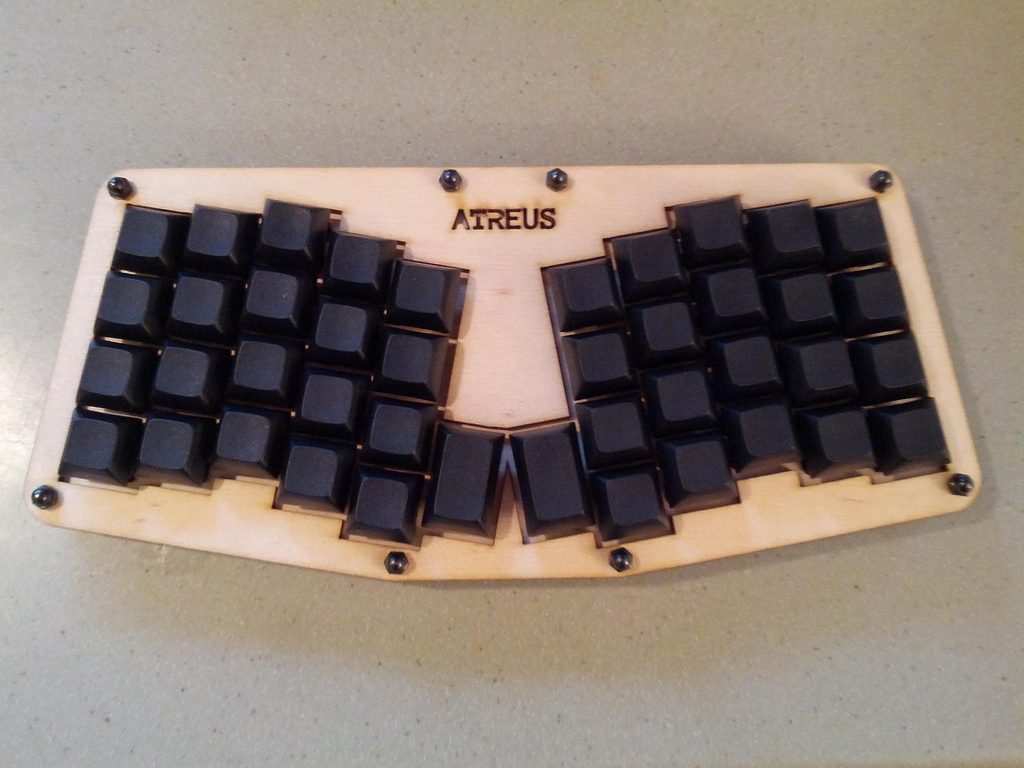
\includegraphics[width=\linewidth]{finished.jpg}}

\end{document}
